\documentclass[addpoints]{exam}
\usepackage{amsmath}
\usepackage{amsfonts}
\usepackage{amssymb}
\usepackage[most]{tcolorbox}
\usepackage{tikz}
\usepackage{pgfplots}
\usepackage{mdframed}
\usepackage{hyperref}
\usepackage{amsthm}
\usepackage{xcolor}
\usepackage{cancel}

\usetikzlibrary{decorations.markings}

\marksnotpoints
\pointsinrightmargin
\bracketedpoints
\printanswers

\hypersetup{
  colorlinks=true,
  linkcolor=blue,
  filecolor=magenta,
  urlcolor=blue,
  pdfpagemode=FullScreen,
}

\renewcommand\qedsymbol{$\blacksquare$}
\newtheorem{theorem}{Theorem}

\urlstyle{same}

\pagestyle{headandfoot}
\firstpageheadrule
\runningheadrule
\firstpageheader{Pre Calc Prep}{Limits}{Shah}
\runningheader{Limits Notes}{}{Shah}
\firstpagefooter{}{}{}
\runningfooter{ }{\thepage}{ }

\begin{document}
\begin{tcolorbox}[breakable, title=LIMITS INTRO, colframe=black, sharp corners, colback=white, colbacktitle=white, coltitle=black]
    \Large\textbf{Intro}
    \newline\normalsize Limits are best introduced as the solution to a specific problem: \textbf{the tangent line problem}. What the tangent line problem is looks something like this:
    \begin{tcolorbox}[breakable, title=THE TANGENT LINE PROBLEM, colframe=black, sharp corners, colback=white, colbacktitle=white, coltitle=black]
      Given some function $f(x)$ and a point on $f(x)$, $(a, f(a))$, how can we find a line tangent to $f(x)$ at $(a, f(a))$? Visually we can represent this like so, 
      \vspace{0.1in}
      \newline
      \begin{center}
        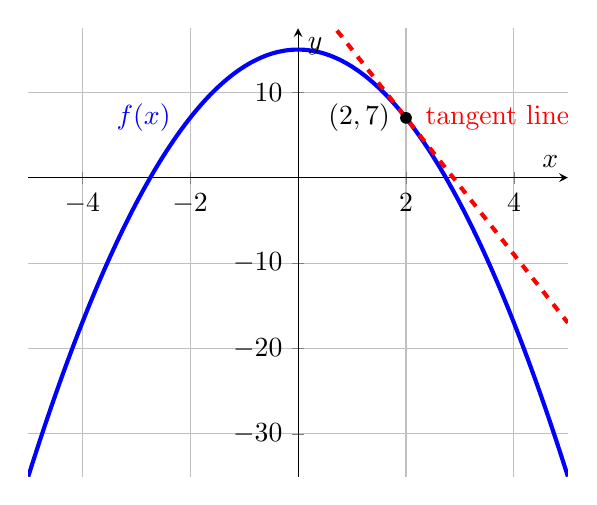
\begin{tikzpicture}
          \begin{axis}[
            axis lines=center,
            grid=both,
            ylabel={$y$},
            xlabel={$x$},
            ymax=17.5
          ]

            \addplot[line width=1.5pt, blue, samples=200]{15-2*x^2};
            \addplot[line width=1.5pt, red, dashed, samples=200]{-8*x + 23};

            \node[circle, fill, inner sep=1.5pt, label={left: $(2, 7)$}] at (axis cs: 2, 7) {};
            \node[label={right: \textcolor{red}{tangent line}}] at (axis cs: 2,  7) {};
            \node[label={left: \textcolor{blue}{$f(x)$}}] at (axis cs: -2,  7) {};
          \end{axis}
        \end{tikzpicture}
      \end{center}
      Where our function is \textcolor{blue}{$f(x)$} and we are trying to find the \textcolor{red}{red} dashed line.
    \end{tcolorbox}
    Let's jump into an example to start! 
    \newline\small \textit{*Recall that tangent simply means 'touching at a single point'\footnote{there are exceptions to this definition}} \normalsize
  \end{tcolorbox}
  \vspace{0.1in}
  \begin{questions}
    \question Find the tangent line to the function $f(x)=15-2x^2$ at $x=2$ \\
    \ifprintanswers
      First, lets begin with a graph of our function, (\textit{hint: its the same function as above!})
      \vspace{0.1in}
      \newline
      \begin{minipage}{0.45\linewidth}
      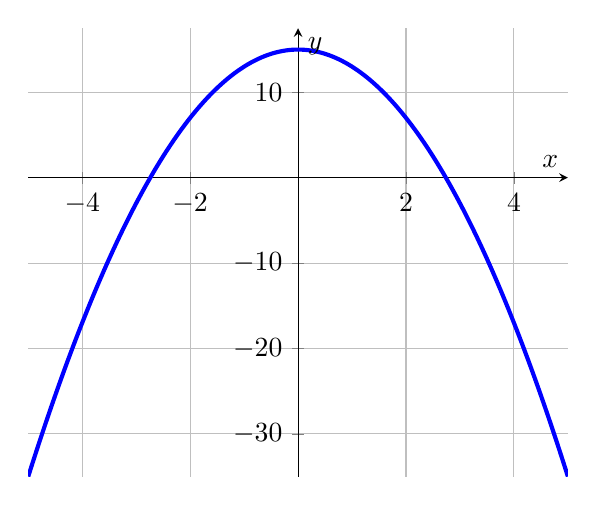
\begin{tikzpicture}
        \begin{axis}[
          axis lines=center,
          grid=both,
          ylabel={$y$},
          xlabel={$x$},
          ymax=17.5
        ]

          \addplot[line width=1.5pt, blue, samples=200]{15-2*x^2};
        \end{axis}
      \end{tikzpicture}
      \end{minipage}
      \hfill 
      \begin{minipage}{0.45\linewidth}
        Now that we have a graph, lets first consider the different parts we need to make a tangent line. We can begin with the \underline{point-slope form of a linear equation}:
        \[y-y_1 = m(x-x_1)\]
        where $(x_1, y_1)$ is a point on the line and $m$ is the slope of our line. Now, thinking back to the problem statement and the definition of "tangent" we might realize that we actually know a point on our line! If we want our tangent line to touch only at a single point on our graph and we know which point we want it to be tangent to, we can simply use that point in our point slope equation!
      \end{minipage}
      \newpage 
      \large\textbf{\underline{ex1.} (sol cont.):} \normalsize So, our point will be $({2}, {7})$. Thus, we can update our equation as follows
      \[
        y-7 = m(x-2)
      \]
      Now all that's left is finding the slope of our line. Remembering our algebra one knowledge we know that the slope between two points is 
      \[
        \frac{y_2-y_1}{x_2-x_2} = \frac{f(b)-f(a)}{b-a}
      \]
      Once again, we already know one point we could use, we just need to find a second point...\\ 
      Consider, again our graph and imagine that this time we had a second point to use for our slope equation, lets denote this point $P = (x_p, y_p)$. Now we can use $P$ to estimate our slope by placing $P$ somewhere on $f(x)$ to form a line between our tangent line point and $P$. We can also note that as $x_p$ moves closer to the $x$-coordinate of the tangent line, our estimation becomes more accurate. It is at this point that I will spoil the correct answer for you in order for you to better grasp what is actually occuring here: in the exact tangent line, our slope is $m=8$. This process can be illustrated with the below graphs: 
      \vspace{0.1in}
      \newline
      \begin{minipage}{0.31\linewidth}
        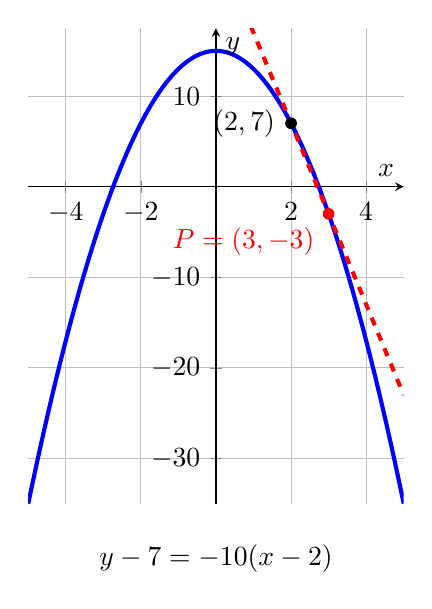
\begin{tikzpicture}
          \begin{axis}[
            title={$y-7=-10(x-2)$},
            title style = {
              at={(0.5, -0.1)},
              anchor=north
            },
            axis lines = center,
            grid = both,
            xlabel={$x$},
            ylabel={$y$},
            ymax=17.5,
            height=3in,
            width=2.5in
          ]

            \addplot[line width=1.5pt, samples=200, blue]{15-2*x^2};
            \addplot[line width=1.5pt, samples=200, red, dashed]{-10*x+27};
            \node[circle, fill, inner sep=1.5pt, label={left: $(2, 7)$}] at (axis cs: 2, 7) {};
            \node[circle, fill, red, inner sep=1.5pt, label={below left: $\textcolor{red}{P=(3, -3)}$}] at (axis cs: 3, -3) {};
          \end{axis}
        \end{tikzpicture}
      \end{minipage}
      \hfill 
      \begin{minipage}{0.31\linewidth}
        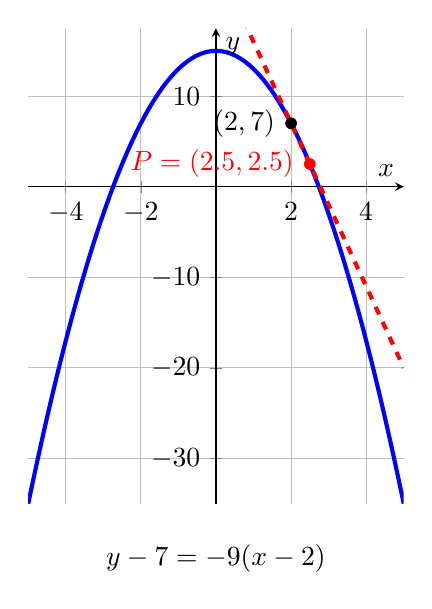
\begin{tikzpicture}
          \begin{axis}[
            title={$y-7=-9(x-2)$},
            title style = {
              at={(0.5, -0.1)},
              anchor=north
            },
            axis lines = center,
            grid = both,
            xlabel={$x$},
            ylabel={$y$},
            height=3in,
            width=2.5in,
            ymax=17.5
          ]

            \addplot[line width=1.5pt, samples=200, blue]{15-2*x^2};
            \addplot[line width=1.5pt, samples=200, red, dashed]{-9*x+25};
            \node[circle, fill, inner sep=1.5pt, label={left: $(2, 7)$}] at (axis cs: 2, 7) {};
            \node[circle, fill, inner sep=1.5pt, red, label={left: $\textcolor{red}{P=(2.5, 2.5)}$}] at (axis cs: 2.5, 2.5) {};
          \end{axis}
        \end{tikzpicture}
      \end{minipage}
      \hfill 
      \begin{minipage}{0.31\linewidth}
        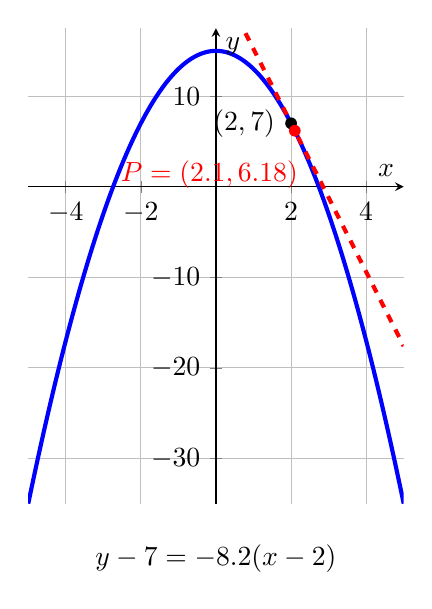
\begin{tikzpicture}
          \begin{axis}[
            title={$y-7=-8.2(x-2)$},
            title style = {
              at={(0.5, -0.1)},
              anchor=north
            },
            axis lines = center,
            grid = both,
            xlabel={$x$},
            ylabel={$y$},
            ymax=17.5,
            height=3in,
            width=2.5in
          ]

            \addplot[line width=1.5pt, samples=200, blue]{15-2*x^2};
            \addplot[line width=1.5pt, samples=200, red, dashed]{-8.2*x+23.4};
            \node[circle, fill, inner sep=1.5pt, label={left: $(2, 7)$}] at (axis cs: 2, 7) {};
            \node[red, circle, fill, inner sep=1.5pt, label={[yshift=-0.2cm, xshift=0.22cm]below left: $\textcolor{red}{P=(2.1, 6.18)}$}] at (axis cs: 2.1, 6.18) {};
          \end{axis}
        \end{tikzpicture}
      \end{minipage}
      \vspace{0.1in}
      \newline
      So, as we moved our point $P$ closer to the $x$-coordinate of $x=2$ our slope approximation got better and our line seemed to become "more tangent"(?) to the graph. It is important to note that we could've easily done this process with points that were to the left of $x=2$ as opposed to the right and, in fact, we really should check the behavior of the the points to the left of $x=2$; however, for the sake of time we won't do that and you'll just have to trust me that it would behave the same as the points to the right. We can generalize this process by generalizing our slope formula: 
      \[
        m = \frac{f(h)-f(2)}{h-2} = \frac{15-2h^2 - 7}{h-2} = \frac{8-2h^2}{h-2}
      \]
      and then substituting into our point slope equation: 
      \[
        y-7=\frac{8-2h^2}{h-2}\left(x-2\right)
      \]
      Now, using all this as evidence it seems that the slope of the line tends towards $-8$ as we move towards $x=2$. As stated earlier, this is the correct answer and is something we will be able to prove later. Thus, our final answer is 
      \[
        \boxed{y-7=-8(x-2)=-8x+23}
      \]
    \else
      First, lets begin with a graph of our function, (\textit{hint: its the same function as above!})
      \vspace{0.1in}
      \newline
      \begin{minipage}{0.45\linewidth}
      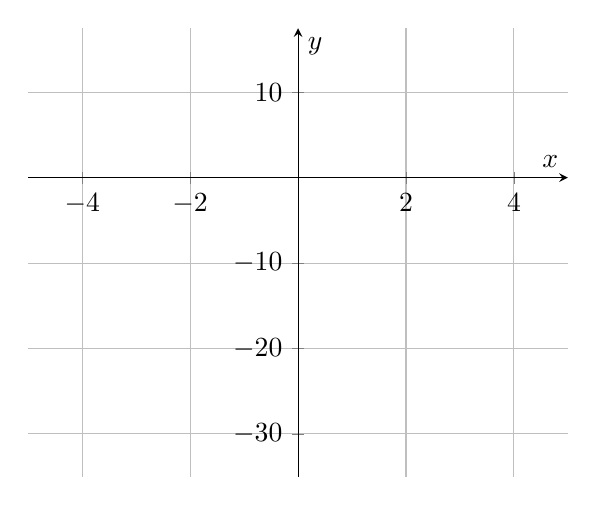
\begin{tikzpicture}
        \begin{axis}[
          axis lines=center,
          grid=both,
          ylabel={$y$},
          xlabel={$x$},
          ymax=17.5
        ]

          \addplot[draw=none, line width=1.5pt, blue, samples=200]{15-2*x^2};
        \end{axis}
      \end{tikzpicture}
      \end{minipage}
      \hfill 
      \begin{minipage}{0.45\linewidth}
        Now that we have a graph, lets first consider the different parts we need to make a tangent line. We can begin with the \underline{point-slope form of a linear equation}:
        \[y-y_1 = m(x-x_1)\]
        where $(x_1, y_1)$ is a point on the line and $m$ is the slope of our line. Now, thinking back to the problem statement and the definition of "tangent" we might realize that we actually know a point on our line! If we want our tangent line to touch only at a single point on our graph and we know which point we want it to be tangent to, we can simply use that point in our point slope equation!
      \end{minipage}
      \newpage 
      \large\textbf{\underline{ex1.} (sol cont.):} \normalsize So, our point will be $(\underline{\hspace{0.3in}}, \underline{\hspace{0.3in}})$. Thus, we can update our equation as follows
      \[
        y-\underline{\hspace{0.3in}} = m(x-\underline{\hspace{0.3in}})
      \]
      Now all that's left is finding the slope of our line. Remembering our algebra one knowledge we know that the slope between two points is 
      \[
        \frac{y_2-y_1}{x_2-x_2} = \frac{f(b)-f(a)}{b-a}
      \]
      Once again, we already know one point we could use, we just need to find a second point...\\ 
      Consider, again our graph and imagine that this time we had a second point to use for our slope equation, lets denote this point $P = (x_p, y_p)$. Now we can use $P$ to estimate our slope by placing $P$ somewhere on $f(x)$ to form a line between our tangent line point and $P$. We can also note that as $x_p$ moves closer to the $x$-coordinate of the tangent line, our estimation becomes more accurate. It is at this point that I will spoil the correct answer for you in order for you to better grasp what is actually occuring here: in the exact tangent line, our slope is $m=8$. This process can be illustrated with the below graphs: 
      \vspace{0.1in}
      \newline
      \begin{minipage}{0.31\linewidth}
        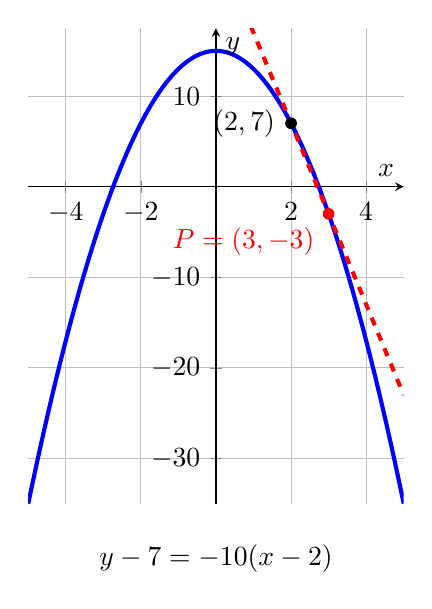
\begin{tikzpicture}
          \begin{axis}[
            title={$y-7=-10(x-2)$},
            title style = {
              at={(0.5, -0.1)},
              anchor=north
            },
            axis lines = center,
            grid = both,
            xlabel={$x$},
            ylabel={$y$},
            ymax=17.5,
            height=3in,
            width=2.5in
          ]

            \addplot[line width=1.5pt, samples=200, blue]{15-2*x^2};
            \addplot[line width=1.5pt, samples=200, red, dashed]{-10*x+27};
            \node[circle, fill, inner sep=1.5pt, label={left: $(2, 7)$}] at (axis cs: 2, 7) {};
            \node[circle, fill, red, inner sep=1.5pt, label={below left: $\textcolor{red}{P=(3, -3)}$}] at (axis cs: 3, -3) {};
          \end{axis}
        \end{tikzpicture}
      \end{minipage}
      \hfill 
      \begin{minipage}{0.31\linewidth}
        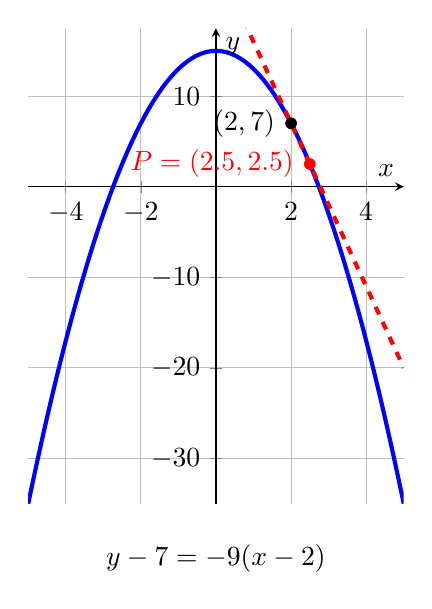
\begin{tikzpicture}
          \begin{axis}[
            title={$y-7=-9(x-2)$},
            title style = {
              at={(0.5, -0.1)},
              anchor=north
            },
            axis lines = center,
            grid = both,
            xlabel={$x$},
            ylabel={$y$},
            height=3in,
            width=2.5in,
            ymax=17.5
          ]

            \addplot[line width=1.5pt, samples=200, blue]{15-2*x^2};
            \addplot[line width=1.5pt, samples=200, red, dashed]{-9*x+25};
            \node[circle, fill, inner sep=1.5pt, label={left: $(2, 7)$}] at (axis cs: 2, 7) {};
            \node[circle, fill, inner sep=1.5pt, red, label={left: $\textcolor{red}{P=(2.5, 2.5)}$}] at (axis cs: 2.5, 2.5) {};
          \end{axis}
        \end{tikzpicture}
      \end{minipage}
      \hfill 
      \begin{minipage}{0.31\linewidth}
        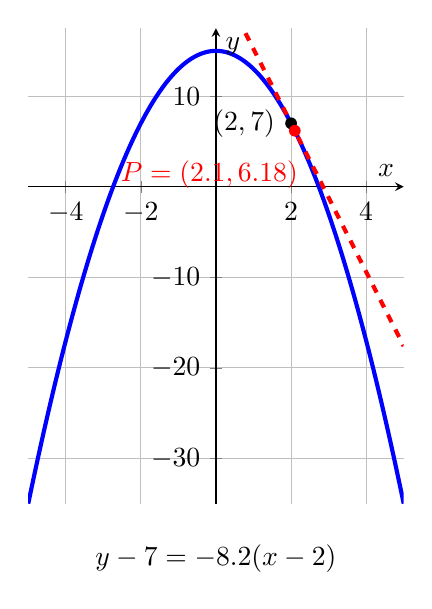
\begin{tikzpicture}
          \begin{axis}[
            title={$y-7=-8.2(x-2)$},
            title style = {
              at={(0.5, -0.1)},
              anchor=north
            },
            axis lines = center,
            grid = both,
            xlabel={$x$},
            ylabel={$y$},
            ymax=17.5,
            height=3in,
            width=2.5in
          ]

            \addplot[line width=1.5pt, samples=200, blue]{15-2*x^2};
            \addplot[line width=1.5pt, samples=200, red, dashed]{-8.2*x+23.4};
            \node[circle, fill, inner sep=1.5pt, label={left: $(2, 7)$}] at (axis cs: 2, 7) {};
            \node[red, circle, fill, inner sep=1.5pt, label={[yshift=-0.2cm, xshift=0.22cm]below left: $\textcolor{red}{P=(2.1, 6.18)}$}] at (axis cs: 2.1, 6.18) {};
          \end{axis}
        \end{tikzpicture}
      \end{minipage}
      \vspace{0.1in}
      \newline
      So, as we moved our point $P$ closer to the $x$-coordinate of $x=2$ our slope approximation got better and our line seemed to become "more tangent"(?) to the graph. It is important to note that we could've easily done this process with points that were to the left of $x=2$ as opposed to the right and, in fact, we really should check the behavior of the the points to the left of $x=2$; however, for the sake of time we won't do that and you'll just have to trust me that it would behave the same as the points to the right. We can generalize this process by generalizing our slope formula: 
      \[
        m = \frac{f(h)-f(2)}{h-2} = \frac{15-2h^2 - 7}{h-2} = \frac{8-2h^2}{h-2}
      \]
      and then substituting into our point slope equation: 
      \[
        y-7=\frac{8-2h^2}{h-2}\left(x-2\right)
      \]
      Now, using all this as evidence it seems that the slope of the line tends towards $-8$ as we move towards $x=2$. As stated earlier, this is the correct answer and is something we will be able to prove later. Thus, our final answer is 
      \[
        \boxed{y-7=-8(x-2)=-8x+23}
      \]
    \fi
  \end{questions}
  \newpage 
  \noindent Now, before we can formally define the limit we must first talk for a second about notation. In example 1, we moved our point $P$ closer to $x=2$ by a certain distance each time. We can represent this by saying that $P=(2+h, f(2+h))$ where $h$ is the distance away from $x=2$. However, often time we won't be dealing with specific points like $x=2$ and often we want to talk in generalaties for any $x$, in this case we can define $P=(x+h, f(x+h))$. Rewriting our slope formula using this new definition of $P$ will give 
    \[
      m = \frac{f(x+h)-f(x)}{x+h-x} = \frac{f(x+h)-f(x)}{h}
    \]
  You should also notice that if we were to let $h=0$ it would result in $\frac{0}{0}$ which is impossible to evaluate due to the division by zero and so is something we \textbf{must} avoid. Remember this!
  \begin{tcolorbox}[breakable, title=DEFINITION OF THE LIMIT, colframe=black, sharp corners, colback=white, colbacktitle=white, coltitle=black]
    We say that the limit of $f(x)$ is $L$ as $x$ approaches $a$ and write this as 
    \[\lim\limits_{x\to\,a} f(x)=L\] 
    provided we can make $f(x)$ as close to $L$ as we want for all $x$ sufficiently close to $a$, from both sides, without actually letting $x$ be $a$.
  \end{tcolorbox}
  \vspace{0.1in}
  \noindent In a less "math speak" way, what our definition is essentially stating is that as $x$ gets closer to $x=a$ (from both sides) then $f(x)$ must be getting closer and closer to $L$. At this point, there are most likely two questions you have: 1. How do I actually evaluate a limit? and 2. How does this help me/relate to the first example? I'd like to start by adressing the first question before the second. \\
  \makebox[\linewidth]{\hrulefill}
  \newline\large\textbf{Evaluating Limits:}
  \newline\normalsize When it comes to evaluating limits, there are multiple techniques used and the first one is the most cumbersome, however, it does a really good job at demonstrating what a limit is and what it actually does.
  \begin{tcolorbox}[breakable, title=TABLE EVALUATION, colframe=black, sharp corners, colback=white, colbacktitle=white, coltitle=black]
    Since limits are just checking that $f(x)$ gets closer to $L$ as $x$ approaches $x=a$ we can do this manually by hand. This is best demonstrated with an example: \\
    \underline{\textbf{ex2:}} Evaluate $\lim\limits_{x\to\,1} x^2$ \\
    Now, obviously we know that at $x=1$, $f(x)=x^2$ will be $f(1)=1$ so we can use this as a baseline to check our answer. In order to use the table evaluation, we will create a table of 6 points\footnote{Standard convention is usually to evaluate $f(x)$ at $x \pm 0.1$, $x \pm 0.01$ and $x \pm 0.001$} (three less than our $x$ value and three greater than) and see what our function values are at these points. From here we can then make an assumption about what the limit will be.: \\
    \begin{center}
      \begin{tabular}{|c|c|}
          \hline
          $x$ & $f(x)$ \\
          \hline
          $1-0.1 = 0.9$ & $f(0.9)=(0.9)^2 = 0.81$ \\
          \hline
          $1-0.01 = 0.99$ & $f(0.99)=(0.99)^2 = 0.9801$ \\
          \hline
          $1-0.001 = 0.999$ & $f(0.999)=(0.999)^2 = 0.998001$ \\
          \hline
          $1 + 0.001 = 1.001$ & $f(1.001)=(1.001)^2 = 1.002001$ \\
          \hline
          $1 + 0.01 = 1.01$ & $f(1.01)=(1.01)^2 = 1.0201$ \\
          \hline
          $1 + 0.1 = 1.1$ & $f(1.1)=(1.1)^2 = 1.21$ \\
          \hline
      \end{tabular}
    \end{center}
    So, as our $x$ values tend towards $x=1$ it seems that $f(x)$ also tends to $1$. Thus, 
    \[\boxed{\lim\limits_{x\to\,1} x^2 = 1}\]
  \end{tcolorbox}
  \newpage 
  \begin{questions}
    \question Evaluate $\lim\limits_{x\to\,2} x^2 - 2$ using a table
    \begin{solution}[2.5in]
      \begin{minipage}{0.45\linewidth}
        \begin{tabular}{|c|c|}
          \hline
          $x$ & $f(x)=x^2-2$ \\
          \hline
          $2-0.1 = 1.9$ & $f(1.9) = 1.61$ \\
          \hline
          $2-0.01 = 1.99$ & $f(1.99) = 1.9601$ \\
          \hline
          $2-0.001 = 1.999$ & $f(1.999) = 1.996001$ \\
          \hline
          $2 + 0.001 = 2.001$ & $f(2.001) = 2.004001$ \\
          \hline
          $2 + 0.01 = 2.01$ & $f(2.01) = 2.0401$ \\
          \hline
          $2 + 0.1 = 2.1$ & $f(2.1) = 2.41$ \\
          \hline
        \end{tabular}
      \end{minipage}
      \hfill
      \begin{minipage}{0.45\linewidth}
        \[\boxed{\lim\limits_{x\to\,2}x^2-2=2}\]
      \end{minipage}
    \end{solution}
  \end{questions}
  \begin{tcolorbox}[breakable, title=DIRECT SUBSTITUTION, colframe=black, sharp corners, colback=white, colbacktitle=white, coltitle=black]
    Direct substitution is the method of evaluting limits that's the most straight forward (in my opinion) and the one that makes the most sense. Direct substituion is simply when if asked to evaluate $\lim\limits_{x\to,a} f(x)$ we just find $f(a)$ and say $L=f(a)$. \textbf{However}, there is one major flaw with direct substitution and that is that it doesn't account for what actually occurs \textit{around} $x=a$ which is what the limit actually tells us. So, you must be sure that the function (graph) actually agrees with the resulting value from your direct substitution.
  \end{tcolorbox}
  \begin{questions}
    \question Evaluate $\displaystyle\,\lim\limits_{x\to\,3} \frac{x^2-2x+2}{x+3}$ 
    \begin{solution}[2.5in]
      We can begin by identifying that our $\displaystyle\, f(x)=\frac{x^2-2x+2}{x+3}$ and our $a=3$. Next,
      \begin{align*}
        f(x) &= \frac{x^2-2x+2}{x+3} \\
        \implies f(a) &= f(3) = \frac{3^2-2(3)+2}{3+3} \\ 
        &= \frac{9-6+2}{6} = \frac{5}{6} \\ 
        &\implies \boxed{\lim\limits_{x\to\,3} \frac{x^2-2x+2}{x+3} = \frac{5}{6}}
      \end{align*}
    \end{solution}
  \end{questions}

  \newpage 

  \begin{tcolorbox}[breakable, title=GRAPHICALLY, colframe=black, sharp corners, colback=white, colbacktitle=white, coltitle=black]
    As we've been working so far, you probably have noticed that there are a lot of refrences to the graphs of functions. This is well because limits can often be evaluated by simply looking at the graph of a function and checking what the behavior is around $x=a$. The major flaw here is that it might not always be easy to graph any given function without a calculator.
  \end{tcolorbox}

  \begin{questions}
    \question Evaluate $\displaystyle\,\mathop {\lim }\limits_{x \to 2} g\left( x \right)\hspace{0.05in}{\mbox{where,}}\hspace{0.1in}g\left( x \right) = \left\{ \begin{array}{ll}\displaystyle \frac{{{x^2} + 4x - 12}}{{{x^2} - 2x}} & {\mbox{if }}x \ne 2\\ 6 & {\mbox{if }}x = 2\end{array} \right.$ \small\textit{(use a calculator/desmos!)}\normalsize
    \begin{solution}[2.5in]
      \begin{minipage}{0.45\linewidth}
        A quick direct substitution might lead us to incorrectly believe that $L=g(2)=6$, however, this is the wrong answer. A quick glance at the graph of $g(x)$ would clearly show us that as $x$ approaches $x=2$ our function does \textbf{not} approach $g(x)=6$. Yet trying to find the behavior \textit{around} $x=2$ by substituting into the other part of the function would yield $\frac{0}{0}$ which we know is impossible and so there must be another way to determine the limit. Revisiting the graph and physically looking at the graph around $x=2$ shows us that $L=\lim\limits_{x\to\,2} g(x) = 4$. Should we have wanted, this also could've been double checked with a table. 
      \end{minipage}
      \hfill 
      \begin{minipage}{0.45\linewidth}
        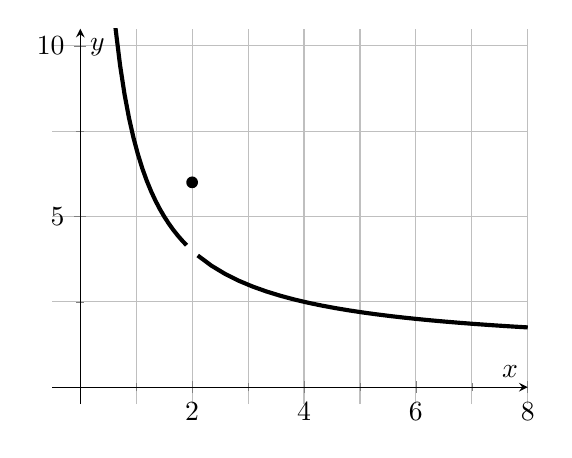
\begin{tikzpicture}
          \begin{axis}[
            grid=both,
            axis lines = center,
            xlabel={$x$},
            ylabel={$y$},
            minor tick num = 1,
            ymax=10.5,
            ymin=-0.5,
            xmin=-0.5,
            height=2.5in,
            width=3in
          ]
            \addplot[line width=1.5pt, black, domain=0:1.9]{(x^2+4*x-12)/(x^2-2*x)};
            \addplot[line width=1.5pt, black, domain=2.1:8]{(x^2+4*x-12)/(x^2-2*x)};

            \node[circle, fill, inner sep=1.5pt, black] at (axis cs: 2, 6) {};
          \end{axis}
        \end{tikzpicture}
      \end{minipage}
    \end{solution}
  \end{questions}
  \begin{tcolorbox}[breakable, title=FACTORING, colframe=black, sharp corners, colback=white, colbacktitle=white, coltitle=black]
    Our final method of evaluating limits is simply just an added layer to direct substitution. There may be time in which direct substitution alone will yield an indeterminate/impossible form such as $\frac{0}{0}$ or division by $0$ in general, however, this doesn't always mean that direct substitution is not the way to go - oftentimes a bit of algebraic manipulation can go a long ways. This, like most things as of late, is best seen through an example.
  \end{tcolorbox}
  \begin{questions}
    \question Evaluate $\displaystyle\, \lim\limits_{x\to\,-3} \frac{x^2+10x+21}{x+3}$
    \begin{solution}[2.5in]
      Since this is the example problem for the factoring section, looking to find something to factor is probably a smart idea; however, for sake of the example let's try direct substitution to start. 
      \[
        \lim\limits_{x\to\,-3}\frac{x^2+10x+21}{x+3} = \lim\limits_{x\to\,-3}\frac{\left(-3\right)^2 + 10(-3) + 21}{-3+3} = \frac{0}{0}
      \]
      So, as promised direct substitution didn't help us at all. Let's try factoring:
      \begin{align*}
        \lim\limits_{x\to\,-3}\frac{x^2+10x+21}{x+3} &= \lim\limits_{x\to\,-3}\frac{\left(x+3\right)\left(x+7\right)}{x+3} \\ 
        &= \lim\limits_{x\to\,-3}\frac{\cancel{\left(x+3\right)}\left(x+7\right)}{\cancel{x+3}} \\
        &= \boxed{\lim\limits_{x\to\,-3}x+7 = -4} \tag{direct substitution}
      \end{align*}
    \end{solution}
  \end{questions}
\end{document}
